\section{Causal Counterfactual Explanation}\label{sec:Causality}
Despite the demand for causality, current standard machine learning models that based on connectivism do not offer a distinction between association and causality \cite{diffThatMakesDiff}. Therefore, causal constraints cannot be learned from training data alone, and often need extra information \cite{bookCausality,preservingCausal}.
\subsection{Structural Causal Model Method}
One of the methods to include causality in the model is directed graph \cite{algorithmicrecourse}. The main idea is to introduce hidden variables to decouple the direct connection between data features and the final prediction. Each feature can only influence one hidden variable, and prediction is based on exclusively these hidden variables. In the context of a directed graph, these hidden variables are called endogenous variables because they have at least one parent node. Exogenous variables are those root nodes without parent nodes, hence are the features. In this way, causal knowledge of feature relations could be applied to the model, \autoref{fig:directedGraph} is an example.
\begin{figure}
  \centering
  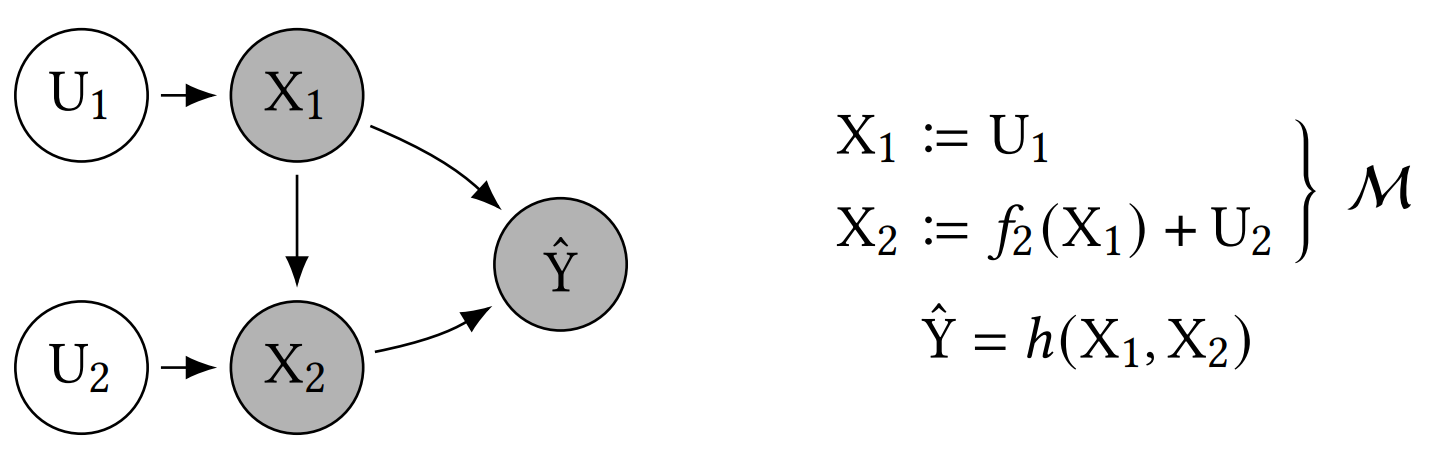
\includegraphics[width=0.5\textwidth]{directedGraph.PNG}
  \caption{An example of the structural causal model, $\mathcal{M}$. In this example, exogenous variable $U_1$ is an individual's annual salary, $U_2$ is the current bank balance. Endogenous variable $X_1$ equals $U_1$, and $X_2$ is the actual bank balance derived from the fact that people usually save part of their salary to their bank account. $\hat Y$ is the prediction function, predicting whether an individual can receive a loan. Credit:\cite{algorithmicrecourse}}
  \label{fig:directedGraph}
\end{figure}

\citeauthor{algorithmicrecourse} \cite{algorithmicrecourse} argue that nearest CF explanation is founded on two assumptions, which are not always true:

\noindent \textbf{Assumption 1:} a minimal perturbation measured by feature distance directly translates to minimal action.

\noindent \textbf{Assumption 2:} there is a monotonic relation between feature-wise differences and action costs.

These assumptions only hold in a world of independent features. Consider the example in \autoref{fig:directedGraph}. Given that the prediction function is $h=sgn(X_1+5\cdot X_2-\$225,000)$. And an individual has an annual salary of \$75,000 and a bank balance of \$25,000, so that the current prediction result is negative. A nearest CF explanation may suggest an annual salary of \$100,000 or a bank balance of \$30,000 to gain a positive result and encourages the user to satisfy either one of them. However, providing that this individual saves 30\% of the annual salary to the account, namely $X_2=\frac{3}{10}\cdot X_1+U_2$, an increase in salary by \$10,000 to \$85,000 would automatically result in \$3,000 more bank balance, and ensure a positive prediction. In this concrete example, the nearest CF explanation method suggests 33\% or 20\% more effort respectively for salary or bank balance. In contrast, after including causal knowledge, the causal CF explanation method shows that 13\% more effort in salary is already sufficient.

Causal CFs should be proximal to the input data with a combination of minimal semantic feature distance and minimal action cost \cite{algorithmicrecourse,preservingCausal}. To calculate example distance measured by action cost, one needs to first define the rules about how values of endogenous variables are assigned. Exogenous variables are the feature, so their values don't need to be assigned.
\subsubsection{Value Assignment} In general, the assignment of endogenous variables can be written as:
\begin{equation}\label{eq:SCM}
  x_i^{SCF}=\mathbb{I}_{i\in I}\cdot a_i+\mathbb{I}_{i\notin I}\cdot(u_i+f_i(parents(x_i^{SCF})))
\end{equation}
where $x_i^{SCF}$ is the i-th feature of a structural CF, $I$ is the intervene set containing the indexes of variables been directly changed, $a_i$ is the intervene value of a feature, $parents()$ returns the parent endogenous nodes of a variable, and $f_i$ is the function illustrating the influence of the endogenous parent nodes on the variable. In plain words, if a feature is not directly intervened, its endogenous variable is determined by the feature value and the downstream effects from parent nodes jointly. Otherwise, its endogenous variable depends merely on the feature value, and the downstream effects are ignored. Note that it is assumed that one action changes only one feature \cite{algorithmicrecourse}, and one feature maps only one single endogenous variable, so changing a feature value is equivalent to changing endogenous variable value when feature correlation is neglected.

Cancelling the downstream effects may be helpful when the causal effect need to be isolated. Depending on the situation, sometimes an additive intervene is desired when action could only be performed additively. For example, in medical treatment previous actions are irreversible. An alternative of \autoref{eq:SCM} is:
\begin{equation}\label{eq:SCMsoft}
  x_i^{SCF}=\mathbb{I}_{i\in I}\cdot \delta_i+(u_i+f_i(parents(x_i^{SCF})))
\end{equation}
where $\delta_i$ is the perturbation of the feature value. In the equation above, the downstream effect is always considered.

\subsubsection{Distance Measurement} For endogenous variables, the distance is defined as a function depending on the CF values of its parent nodes and its own CF value \cite{preservingCausal}, i.e.
\begin{equation}\label{eq:CausalDist}
  DistCausal(x_i,x_i^{SCF})=Dist(x_i^{SCF},f_i(parents(x_i)))
\end{equation}
note that the factual value of the endogenous value is not included in this equation. For exogenous variables, the distance function is still $L_1$ or $L_2$ norm as usual. The complete distance function becomes:
\begin{equation}\label{eq:CausalDistComplete}
  DistCausalComplete(\textbf{x,c})=\sum_{i\in U}Dist(u_i^{cf},u_i)+\sum_{j\in X}DistCausal(x_j^{cf},x_j)
\end{equation}
And this function can be directly applied in gradient-based method, by replacing the proximity term in \autoref{eq:watcher}. In practice, the full causal graph is often unknown. In this case, only the variables with known causal knowledge are treated as endogenous variables and the rest are treated as exogenous variables \cite{preservingCausal}.

\subsection{Domain Knowledge Method}
Without knowing the true causal functions, one can still approximate causality with domain knowledge by loss function \cite{preservingCausal}. For unary constraints, namely, those features that can only increase or decrease, the following term could be appended:
\begin{equation}\label{eq:approxUnary}
  \pm \min(0,x_i^{cf}-x_i)
\end{equation}
For binary constraints, that two features are monotonically related, either positively or negatively, the appended term could be:
\begin{equation}\label{eq:approxBi}
  +(x_2-\alpha-\beta\cdot x_1)-\min(0,\beta)
\end{equation}
\subsection{Summary of Causal Counterfactual Explanation}
Compared with the mainstream of the nearest CF explanation method, literature about causal CF explanation method is scarce \cite{algorithmicrecourse}. Current research shows that the causal CF method is able to generate feasible explanations, but their application is severely limited, partially because complete causal graphs and structural equations are rarely available in the real world \cite{CFReview}. Moreover, \citeauthor{algorithmicrecourse} \cite{algorithmicrecourse} mentioned that the preliminary limitation of their structural causal graph method is the assumption that one action could only change one feature. However, such actions exist that change multiple features simultaneously. For example, a switch of job changes the income as well as employment length. These factors should be solved with a different causality model.    